\documentclass[12pt]{article} 

% Adjust margining to narrow
\usepackage{geometry}
\geometry{a4paper, total={170mm,257mm}, left=20mm, top=20mm}

% Mathematics font
\usepackage{amsfonts}
\usepackage{amsmath}

% Graphics import
\usepackage{graphicx}
\usepackage{subcaption}
\graphicspath{{C:/Users/user/Desktop/KUL - Mstat/Big Data Platforms and Technologies/report/graph}}

% Advanced table
\usepackage{tabularx}
\usepackage{makecell}

% No indentation
\setlength\parindent{0pt}

% ------------------------------------------------------------------------
% Assignment content
\begin{document}
\begin{titlepage}
	\begin{center}
	\vspace*{1cm}
    
\includegraphics[width=0.4\textwidth]{KUL}\\
	\vspace{2.5cm}
    {\Large Report for Advanced Analytics in Business}
            
    \vspace{1.5cm}

    {\large Cheung Wai Chun, r0817438}\\
    \vspace{0.5cm}
    {\large David Badajkov, r0604517}\\
    \vspace{0.5cm}
    {\large Ana Maria Giraldo Vargas, r0822450}\\
    \vspace{0.5cm}
	{\large Sonia Rocio 	Socadagui Casas, r0823960}\\
	\vspace{0.5cm}
	{\large Marcela 	Lopez Viveros, r0773141}
	\vspace{1.5cm}

       \today
   \end{center}
\end{titlepage}

% ------------------------------------------------------------------------
\newpage
\tableofcontents
\newpage

\section*{Assignment 1}
\addcontentsline{toc}{section}{Assignment 1}


\subsection*{Feature engineering}
\addcontentsline{toc}{subsection}{Feature engineering}

The (training) dataset for Assignment 1 consists of 55463 observations and 78 features. The number of features. It is easy to observe that there are a lot of missing values and categorical or date features in the dataset. In this section, we would discuss the strategies used in handling such problems. 

\subsubsection*{Missing values}
\addcontentsline{toc}{subsubsection}{Missing values}

As shown in figure 1, there are 55 feature which contain missing values, and 24 out of them contain more than 80\% of missing values. For those features with a high proportion of missing values (more than 50\%), missing values are treated as an extra category. By treating missing values as an extra category, the information of the non-missing entries of those features can be retained and learnt by the model, whereas removal of those features may lead to a loss in information or pattern. For those features with a lower proportion of missing values, imputation techniques can be applied to estimate their possible values.

\begin{figure}[h]
\centering
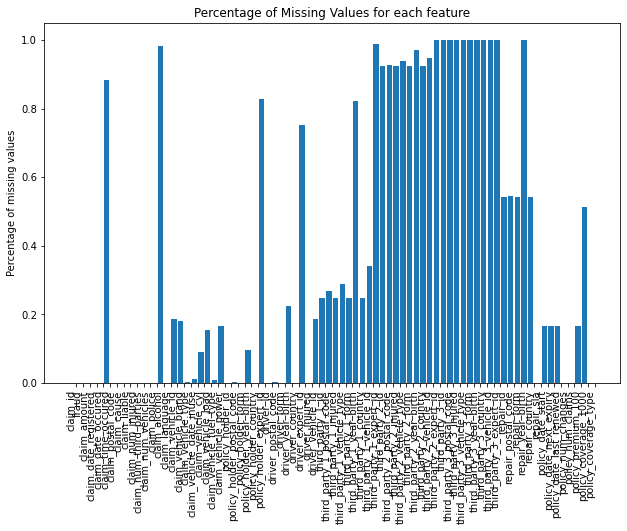
\includegraphics[width=1\linewidth]{missing_value_plt1}
\caption{Proportions of missing values for each feature}
\end{figure}

\clearpage

\subsubsection*{Date features}
\addcontentsline{toc}{subsubsection}{Date features}

Some features are available in form of date. In the dataset, the following features are in terms of date: \texttt{claim\_date\_registered}, \texttt{claim\_date\_occured}, \texttt{claim\_vehicle\_date\_inuse}, \texttt{policy\_date\_start}, \texttt{policy\_date\_next\_expiry} and \texttt{policy\_date\_last\_renewed}. However, date itself is not suitable to serve as an input for some machine learning models. Hence, as summarized in table 1, we construct another set of features which are more interpretable and meaningful based on these date features.\\

Apart from the aforementioned features, features related to birth year are also considered as date features. They are \texttt{policy\_holder\_year\_birth}, \texttt{driver\_year\_birth}, \texttt{third\_party\_1\_year\_birth}, \texttt{third\_party\_2\_year\_birth}, \texttt{third\_party\_3\_year\_birth} and \texttt{repair\_year\_birth} in the dataset. By subtracting them from the year of \texttt{claim\_date\_occured}, we obtain age-related features.

\begin{table}[h]
	\begin{tabular}{|l|p{11.5cm}|}
	\hline
	Constructed features & Descriptions\\
	\hline
	\texttt{days\_before\_registered} & The number of days between \texttt{claim\_date\_registered} and \texttt{claim\_date\_occured}.\\
	\hline
	\texttt{days\_before\_occured} & The number of days between \texttt{claim\_date\_occured} and \texttt{claim\_vehicle\_date\_inuse}.\\
	\hline
	\texttt{policy\_length} & The number of days between \texttt{policy\_date\_last\_renewed} and \texttt{policy\_date\_start}.\\
	\hline
	\texttt{policy\_claim\_length} & The number of days between \texttt{policy\_date\_next\_expiry} and \texttt{claim\_date\_occured}.\\
	\hline
	\end{tabular}
	\caption{Featurization of date features}
\end{table}

\vspace{-1cm}
\subsubsection*{Data quality issue}
\addcontentsline{toc}{subsubsection}{Data quality issue}

During data cleaning process, we discovered some problems with regards to data quality. For example, the instance with claim id 62780 has an invalid value for the year of \texttt{claim\_vehicle\_date\_inuse}. Such observations may be due to input error in manual data entering process. However, they can be hard to observe in general.

\begin{figure}[h]
\centering
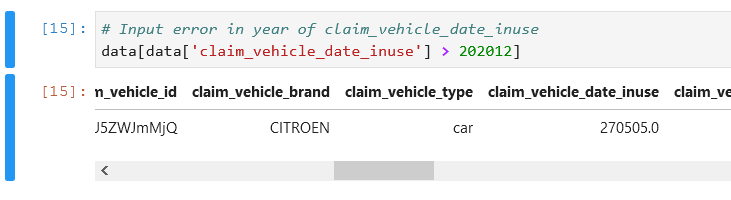
\includegraphics[width=1\linewidth]{data_quality_issue}
\caption{Invalid value of \texttt{claim\_vehicle\_date\_inuse}}
\end{figure}

\vspace{-1cm}
\subsubsection*{Data binning}
\addcontentsline{toc}{subsubsection}{Data binning}

Binning continuous features can help incorporating missing values and extreme values in a more natural way as they can be reformulated as categorical features. It is useful for those continuous features with a high proportion of missing values or highly right-skewed. For age-related features, they are binned by age groups with equal intervals, referencing to their histograms.

\subsection*{Exploratory data analysis}
\addcontentsline{toc}{subsection}{Exploratory data analysis}

\subsection*{Model building}
\addcontentsline{toc}{subsection}{Model building}

\subsection*{Interpretation}
\addcontentsline{toc}{subsection}{Interpretation}

\subsection*{Reflection}
\addcontentsline{toc}{subsection}{Reflection}

\section*{Assignment 2}
\addcontentsline{toc}{section}{Assignment 2}

\section*{Assignment 3}
\addcontentsline{toc}{section}{Assignment 3}

\section*{Assignment 4}
\addcontentsline{toc}{section}{Assignment 4}
\end{document}